\chapter[Planejamento de Desenvolvimento]{Planejamento de Desenvolvimento}
\label{cp:planejamento}

\section{Processo de Desenvolvimento de Software}

Segundo \cite{sommerville}, esse processo pode ser definido como "Um processo de \textit{software} é um conjunto de atividades relacionadas que levam à produção de um produto de \textit{software}."

Neste trabalho, foram definidas as principais atividades a serem realizadas para alcançar o objetivo final de ter um \textit{software} gratuito,código aberto e que auxilie os gerentes a otimizar suas reuniões por meio computacional são:

\begin{itemize}
    \item Especificação do \textit{software}: funcionalidades e restrições do \textit{software};
    \item Projeto e implementação do \textit{software}: as especificações que o \textit{software} deve atender;
    \item Validação de \textit{software}: para que atenda as expectativas do cliente, o \textit{software} deve ser validado pelo mesmo;
    \item Evolução do \textit{software}: o \textit{software} deve ser capaz de ser extensível a mudanças, tendo assim seu código aberto.
\end{itemize}

\section{Linguagem de Software}

Linguagem de programação são instruções passadas de maneira que o computador entenda e apresente um retorno. Existem diversas linguagens de programação, desde a mais baixo a alto nível.

Linguagens de \textit{software}, como também podem ser chamadas, são divididas em duas frentes: \textit{front-end} e \textit{back-end}. Ambas serão explicadas nos tópicos a seguir.

\subsection{Front-end}

A programação de um \textit{software} pelo ponto de vista do \textit{front-end} é a visão final do usuário com o sistema. \textit{Front-end} é a responsável pela interação do usuário com o sistema e essa interação é dada a partir de telas/páginas. Existem diversos tipos de \textit{frameworks} que auxiliam os desenvolvedores a trabalhar com essa frente, como:

\begin{itemize}
    \item \textit{Bootstrap
    \item Materialize
    \item React
    \item Angular 4}
\end{itemize}

A linguagem \textit{front-end} escolhida para este projeto, foi o \textit{React}, pois além de facilitar o desenvolvimento e interação com usuário final, é uma das mais utilizadas ao redor do mundo, então é facilita uma manutenção futura do \textit{software}.

\subsection{Back-end}

A programação \textit{back-end} possui as responsabilidades de receber os dados pelo \textit{React}, que é o \textit{front-end} deste projeto, possui o dever de tratar os dados, valida-los e fomentá-los a visão do usuário.

Existem diversas linguagens \textit{back-end} que auxiliam os desenvolvedores a trabalhar em uma linguagem que o computador entende, como:

\begin{itemize}
    \item \textit{Python Django-Rest
    \item Java
    \item Ruby on Rails
    \item PHP}
\end{itemize}

A linguagem \textit{back-end} escolhida para este projeto, foi a \textit{Python Django-Rest}, pois tem uma ótima conexão com a linguagem \textit{front-end}, e por ser muito utilizada, possibilita assim uma manutenção futura.

\subsection{Arquitetura de Software}

A arquitetura de \textit{software} é como o sistema deve ser organizado com a estrutura geral do projeto. A arquitetura possui um valor alto dentro da construção de um \textit{software}, pois nela se tem o elo entre o projeto e a engenharia de requisitos. Possui o dever identificar os principais componentes estruturais no sistema e o relacionamento entre eles. Neste projeto a arquitetura adotada é uma adaptação ao padrão arquitetural MVC \textit{(model-view-controller)}.

\subsubsection{Model-View-Controller}
\label{sec:mvc}

O padrão arquitetural MVC é responsável de responsabilidades em camadas. A primeira é \textit{Model}(modelo), que é responsável pela manipulação de dados, ou seja, leitura, escrita de dados e também suas validações é de responsabilidade da Model. A segunda camada é a \textit{View}(visão), que possui a responsabilidade de interação com o usuário. Por último se tem a \textit{Controller}(controladora), responsável por receber as aquisições do usuário. A controller também tem o dever de disponibilizar os dados para a \textit{view} e assim ocorrer a interação com o usuário.

\subsubsection{Arquitetura do Projeto}

Neste projeto é feita uma adaptação ao padrão MVC, por conta da escolha da linguagem \textit{front-end}. O \textit{React} possui um padrão arquitetural diferente, chamado de arquitetura de componentes/microserviços. Esse padrão possui semelhanças ao MVC, e o que será utilizado dele será a parte da \textit{View}. Enquanto a linguagem \textit{back-end} é responsável por trabalhar os dados provindos do \textit{front-end} e oferecer um retorno a ele. 

A seguir será mostrado como funciona separadamente o \textit{React},relacionado ao \textit{front-end} que engloba a \textit{View}, enquanto o \textit{Python Django-Rest} é responsável pelo \textit{back-end} e que engloba a \textit{Model} e a \textit{Controller}:

\begin{figure}[H]
	\centering
	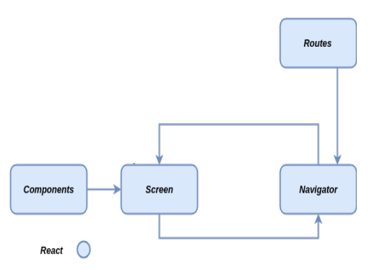
\includegraphics[width=1.0\textwidth]{figuras/diagrama_react.png}
	\caption{Diagrama React/Microsserviços}
	\label{img:diagrama_react}
\end{figure}

\begin{figure}[H]
	\centering
	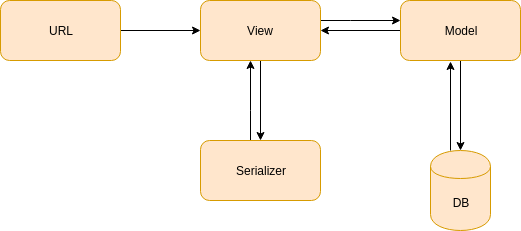
\includegraphics[width=1.0\textwidth]{figuras/django_rest.png}
	\caption{Diagrama Django REST Framework}
	\label{img:diagrama_rest}
\end{figure}

\section{Cronograma TCC}
